\subsection{Использование SimGAN для повышения реалистичности сгенерированных изображений}
Сети SimGAN были созданы Apple в 2017 году\cite{simgan-overview}. Этот подвид генеративно-состязательных сетей направлен на улучшение реалистичности изображений. Отличительной особенностью этих сетей является то, что нет необходимости выделять признаки вручную, описывать характеристики реалистичных данных – обучение происходит на сырых данных и без учителя.

Это достигается благодаря использованию идеи из обычных генеративно-состязательных сетей: сеть должна состоять из двух частей, генератора, который пытается улучшить реалистичность изображения, и дискриминатора, который пытается отличать реальные изображения от сгенерированных. Архитектура SimGAN сети приводится на рисунке \ref{fig:sim-gan}.

\begin{figure}[h]
	\centering
	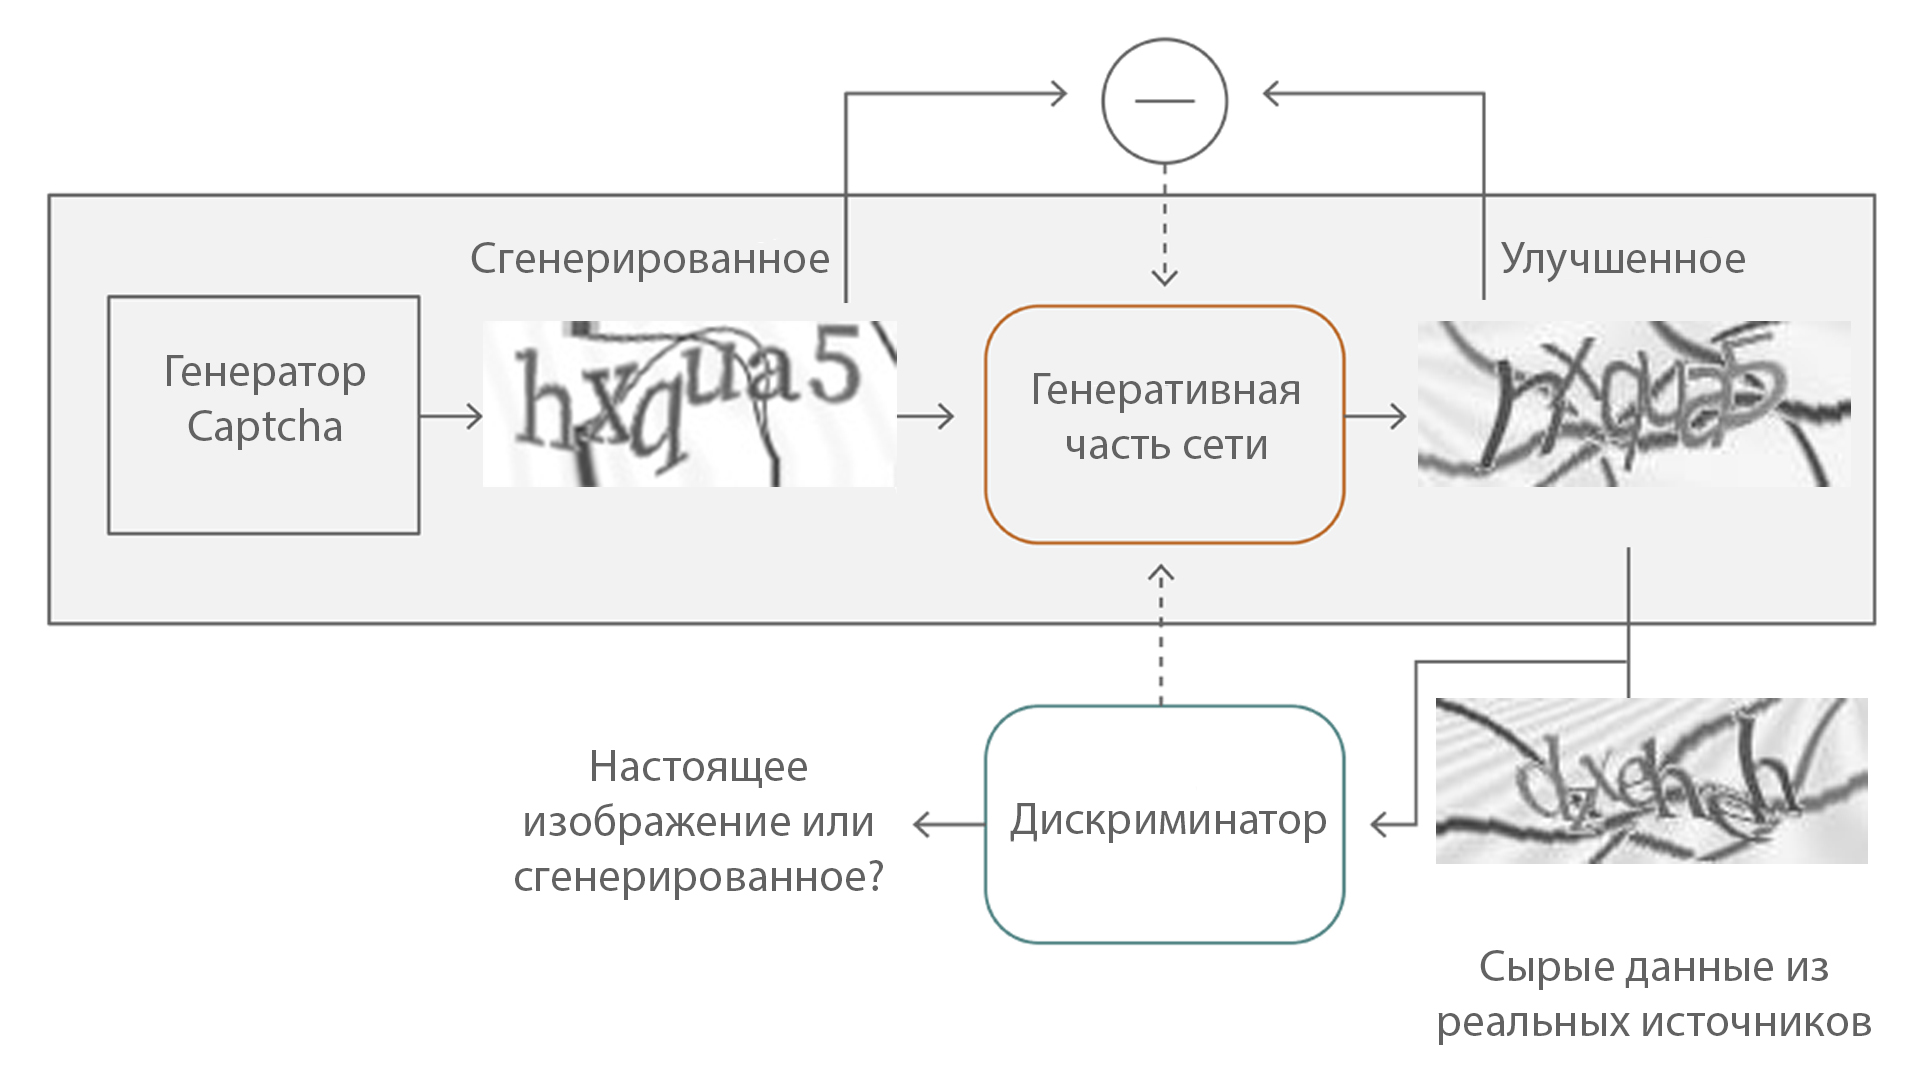
\includegraphics[width=0.8\textwidth]{sim-gan}
	\caption{Структура SimGAN сети.}
	\label{fig:sim-gan}
\end{figure}

Наша цель – обучить сеть, а именно, генеративную ее часть, так, чтобы при подаче на вход сгенерированного изображения на выходе получилось изображение, очень похожее на реальные данные.

Одна из задач, которые ставятся перед SimGAN сетями, является не просто модификация изображений, но и сохранение данных, которые на них изображены. Так, например, в случае работы с картинками captcha, сеть после своей работы должна сохранить то слово, которое было изображено перед обработкой. Это достигается путем дополнения функции потерь элементом регуляризации. В качестве этого элемента мы возьмем обычное расстояние L1, которое будет предотвращать значительные различия между сгенерированными и улучшенными изображениями.
